\documentclass[serif]{beamer}

\usepackage[UTF8,noindent]{ctexcap}
\usepackage{graphicx} 
\usepackage{amsmath}
\title{\textbf{学习工作总结}}%标题
\author{李啟明}%作者
\begin{document}
\begin{frame}[plain]
	\maketitle
\end{frame}

\begin{frame}{学习课程}
    javascript和计算机图形学,目的是通过js绘制图形
    \\[2ex]
    正在学习概率论和数理统计
    \\[2ex]
    学习LaTex
    \\[2ex]
\end{frame}
\begin{frame}{注意力机制}
\qquad 不同的词对文本的贡献是不相同的,对于输入,得到它的各个部分的权重就是Attention的主要目标。
\\[2ex]
\qquad 基于文本的注意力机制如图:
\\[2ex]
	    \begin{center}
    	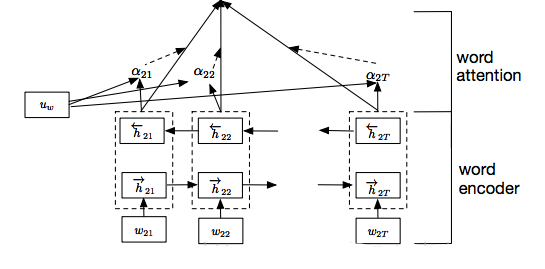
\includegraphics[scale=0.6]{attention.png}
    	\end{center}
    
\end{frame}

\begin{frame}{Attention Mechansim}

	\qquad W为权重矩阵,b为偏置,u的作用是对结果降维,score函数刻画了对应词在句子中的贡献:
	\begin{equation*}
	u_{t}=tanh(W_{w}h_{t}+b_{w})
	\end{equation*}
	\begin{equation*}
	score(t)=u_{t}^{T}u_{w}
	\end{equation*}
	\qquad 句子中第t个词的权值为$\alpha_{t}$:
	\begin{equation*}
	\alpha_{t}=\frac{e^{score(t)}}{\sum_{t}e^{score(t)}}
	\end{equation*}
	\qquad 注意力机制决定了句子中哪些词具有更高的权重,即对文本有更大的贡献。

\end{frame}
\begin{frame}{基于attention的三种模型}
\qquad 考虑在嵌入层之后、卷积层之间和卷积层、池化层之间加入attention层,对输入的向量各自乘上对应的权重$\alpha_t$,得到新的输入。
\\[2ex]
\qquad AttCNN1模型:接受嵌入层输出的词向量矩阵,在attention层为每个词向量计算权重,将加权后的词向量矩阵作为卷积层的输入。
\\[2ex]
\qquad AttCNN2模型:对宽卷积的输出,经过attention层的处理后,作为池化层的输入。
\\[2ex]
\qquad AttCNN3模型:结合前两种模型,同时对嵌入层和卷积层的输出计算attention权重,作为下一层的输入。
\\[2ex]

\qquad 代码实现: \url{https://github.com/liqiming-whu/text-classification}
\end{frame}
\end{document}